% !TeX root = ..\essay.tex

\section{Evaluation}
\label{ch:evaluation}

\subsection{evaluation setting}
To evaluate the summaries they were manually annotated.
Each summary has been annotated by at least four raters with the following criteria:
\begin{table}[H]
	\begin{tabularx}{\textwidth}{l|X} \toprule
		criteria & description \\ \midrule
		Grammaticality      & \\
		Non-Redundancy      & \\
		Referential Clarity & \\
		Focus               & \\
		Structure           & \\
		Coherence           & \\
		Readability         & \\
		Information Content & \\
		Spelling            & \\
		Length              & \\
		Overall Quality     & \\ \bottomrule
	\end{tabularx}
	\caption{evaluation criteria}
	\label{tab:evacriteria}
\end{table}

The score for each criteria was set with the help of a five-point Likert scale.
For each criteria the opportunity to give an estimation in weighting and confidence was be expected, too. These further possibilities to rate a summary are also realized with a five-point Likert scale.
In table~\ref{tab:evalikert} the scales for Score, Weight and Confidence are shown:

\begin{table}[H]
	\begin{tabularx}{\textwidth}{l|XXX} \toprule
		Scale & Score & Weight & Confidence \\ \midrule
		1 & very poor & completely unimportant & very low \\
		2 & poor & unimported & low \\
		3 & barerly acceptable & indifferent & half sure \\
		4 & good & important & high \\
		5 & very good & absplutely important & very high \\ \bottomrule    
	\end{tabularx}
	\caption{Likert scale for Weight and Confidence}
	\label{tab:evalikert}
\end{table}

The annotators had also the opportunity to comment each criteria for each summary with free text.

\subsection{JSD}
To compare the contents of our summaries with the source documents we used the
Jensen Shannon divergence, which we computed with \textit{SIMetrix}, a tool of
Annie Louis \citep{louis}. The scores are generated by considering the vocabulary
distributions of the summaries and the source documents. We cleared the summaries
and original texts of all HTML tags and summary titles and did the same
with the summaries of the other groups and the summaries of the first baseline
that was given to all groups. The result of the tools can be seen in
figure~\ref{fig:jsd}. Note that higher Jensen Shannon divergence scores indicate
summaries of lower quality. As can be seen our values are the third best after
the scores of group 4 and 3.
\begin{figure}[H]
	\centering
	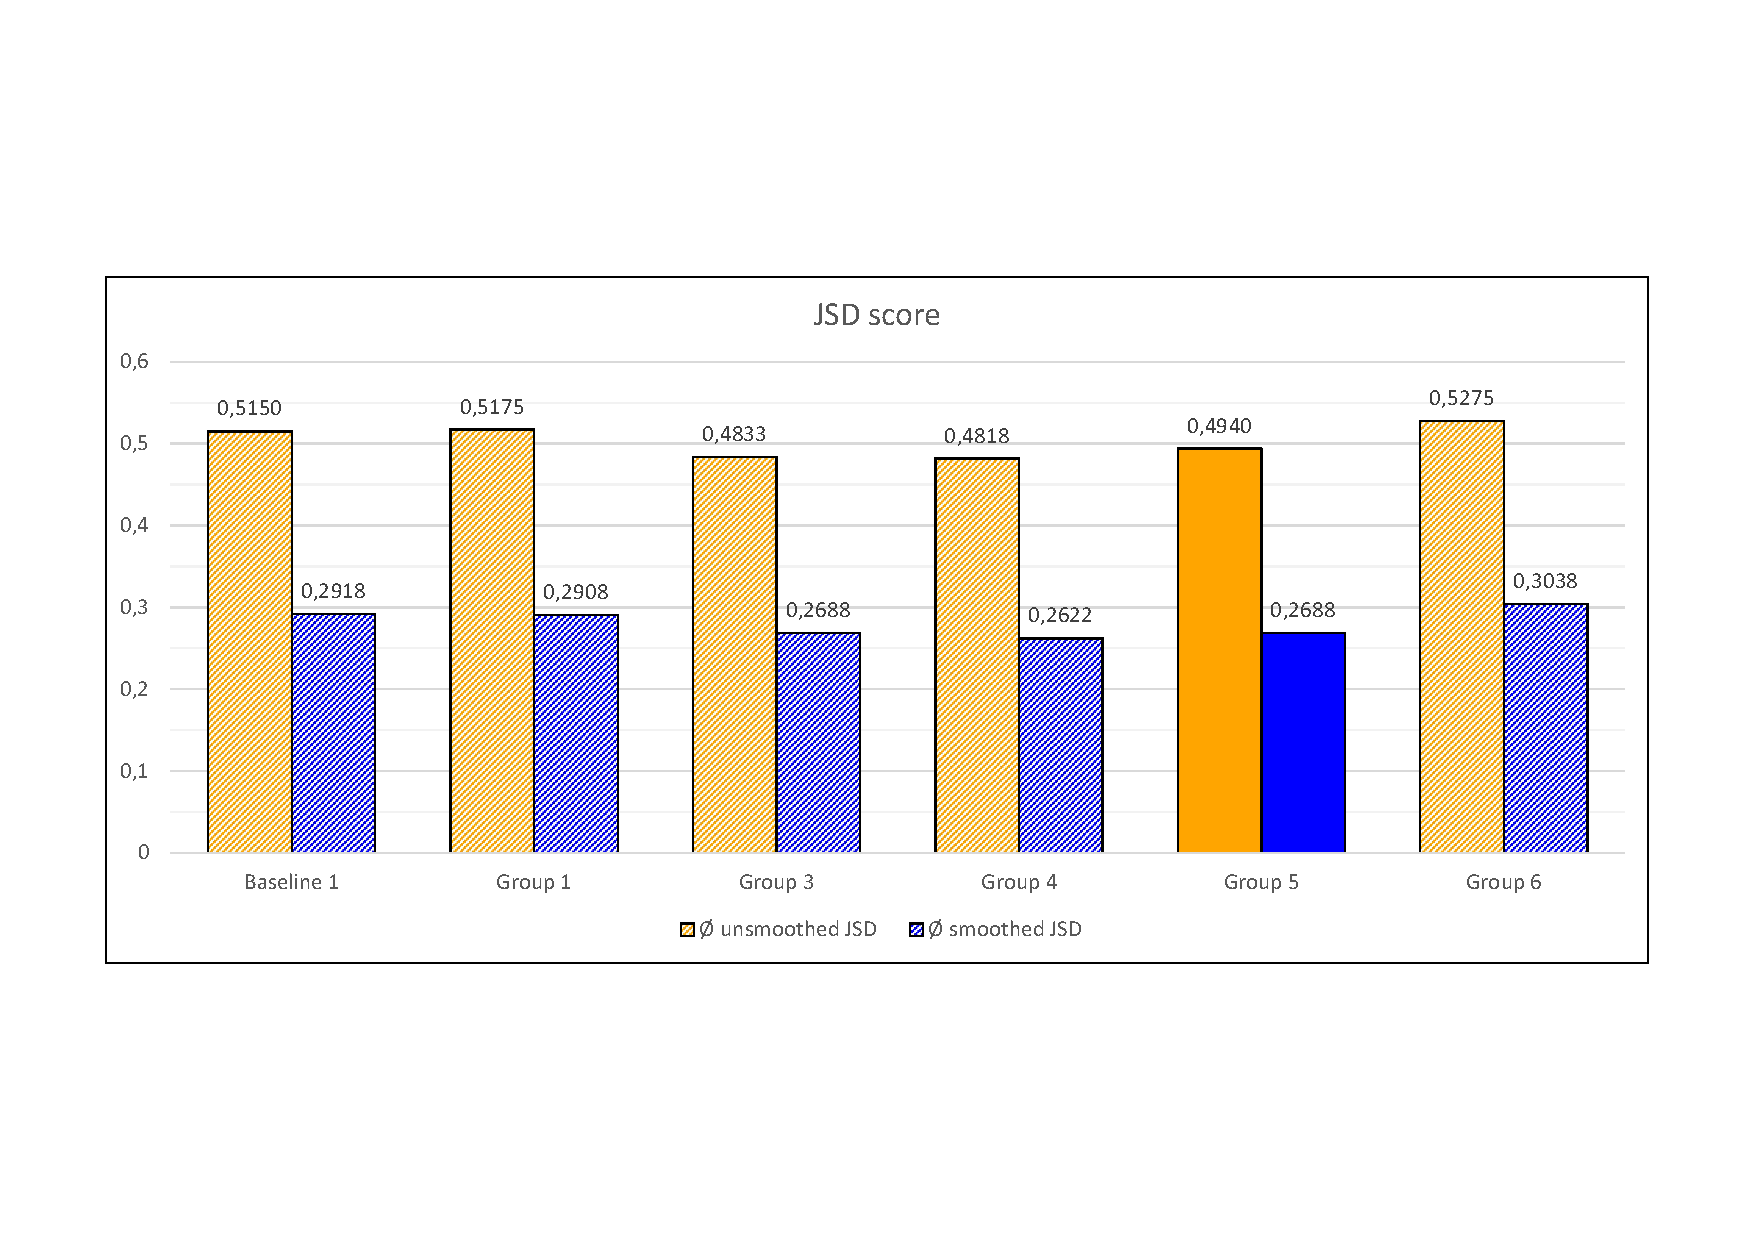
\includegraphics[trim= 0 150 0 150,width=\textwidth]{img/jsd.pdf}
	\caption{JSD score}
	\label{fig:jsd}
\end{figure}


\subsection{Scores per Criteria}

\begin{figure}[H]
	\centering
	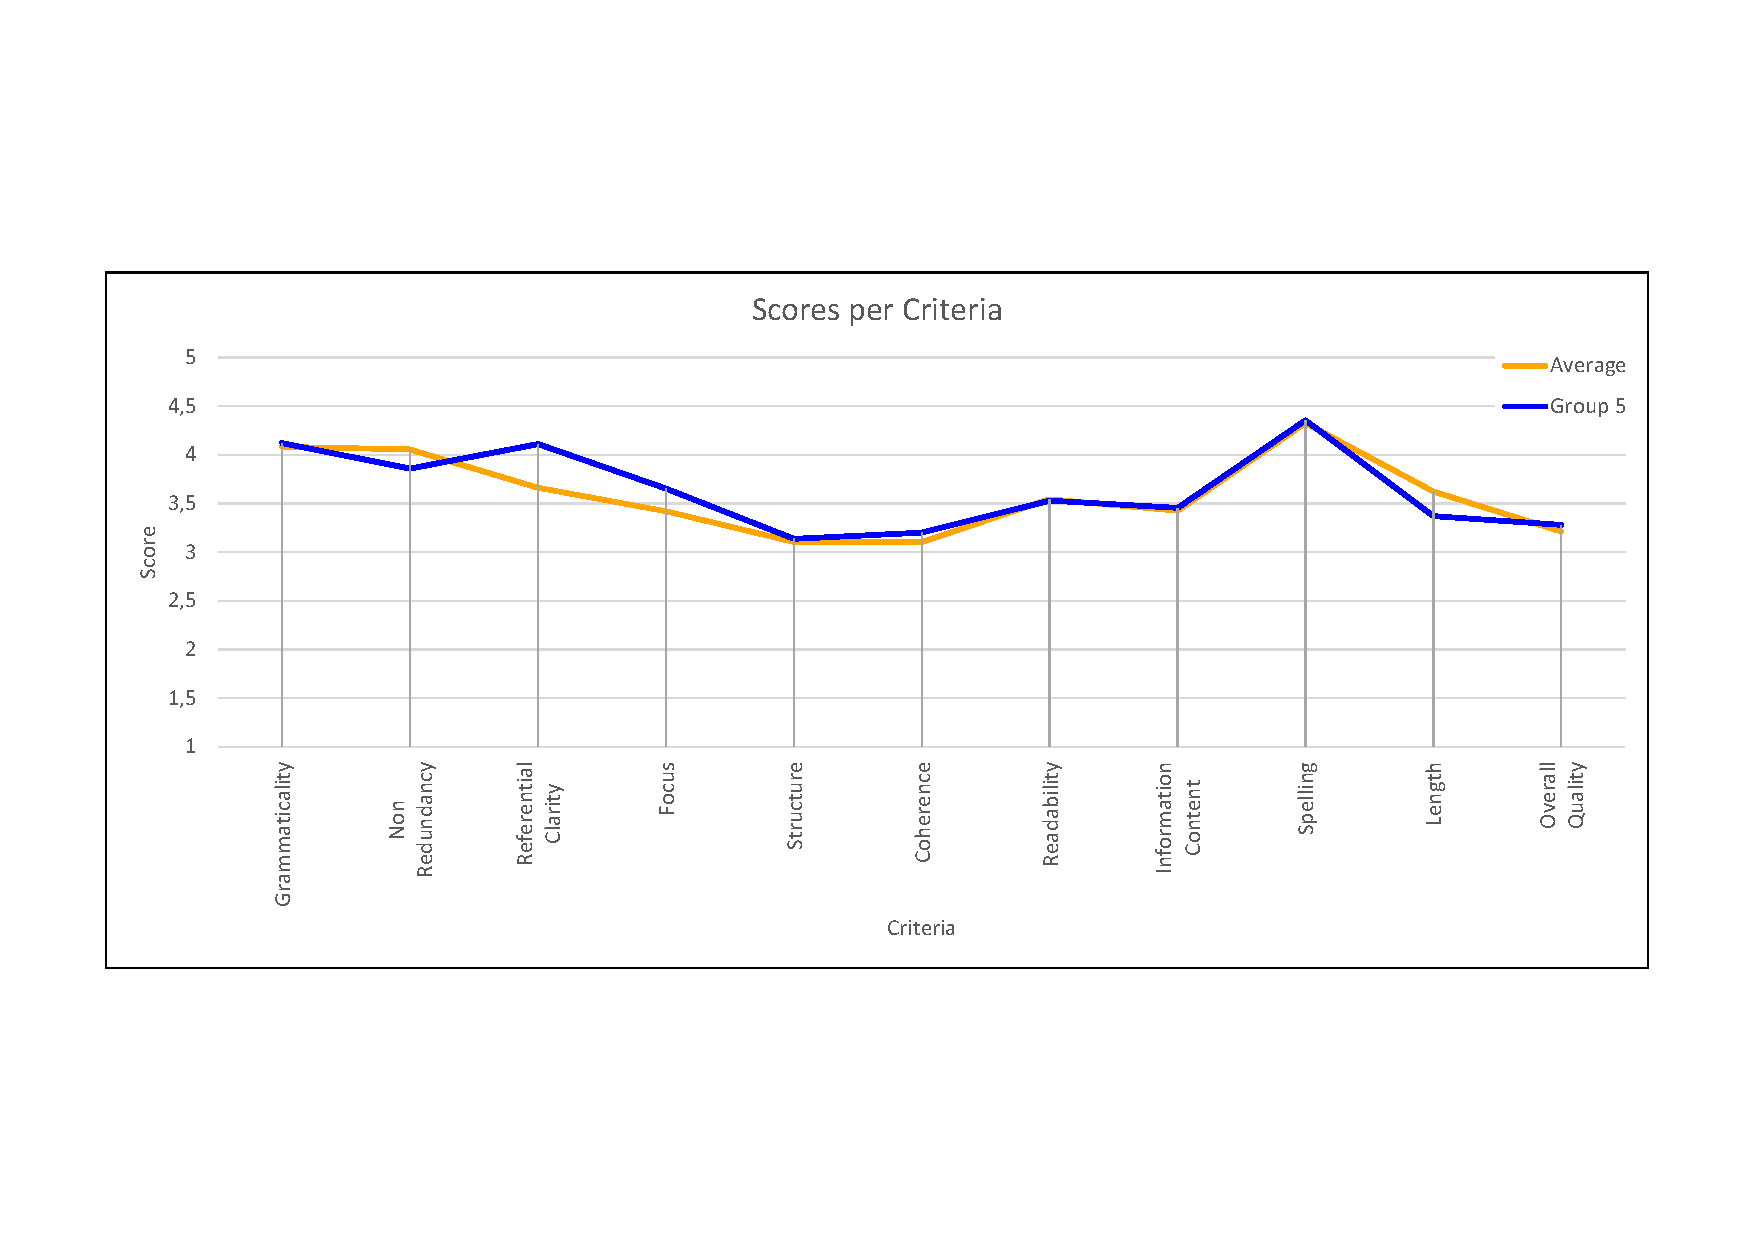
\includegraphics[trim= 0 150 0 150,width=\textwidth]{img/scores_per_criteria.pdf}
	\caption{scores per criteria}
	\label{fig:spc}
\end{figure}

\subsection{why so good / bad}
free text analysis per criteria


\subsection{box plot}

\begin{figure}[H]
	\centering
	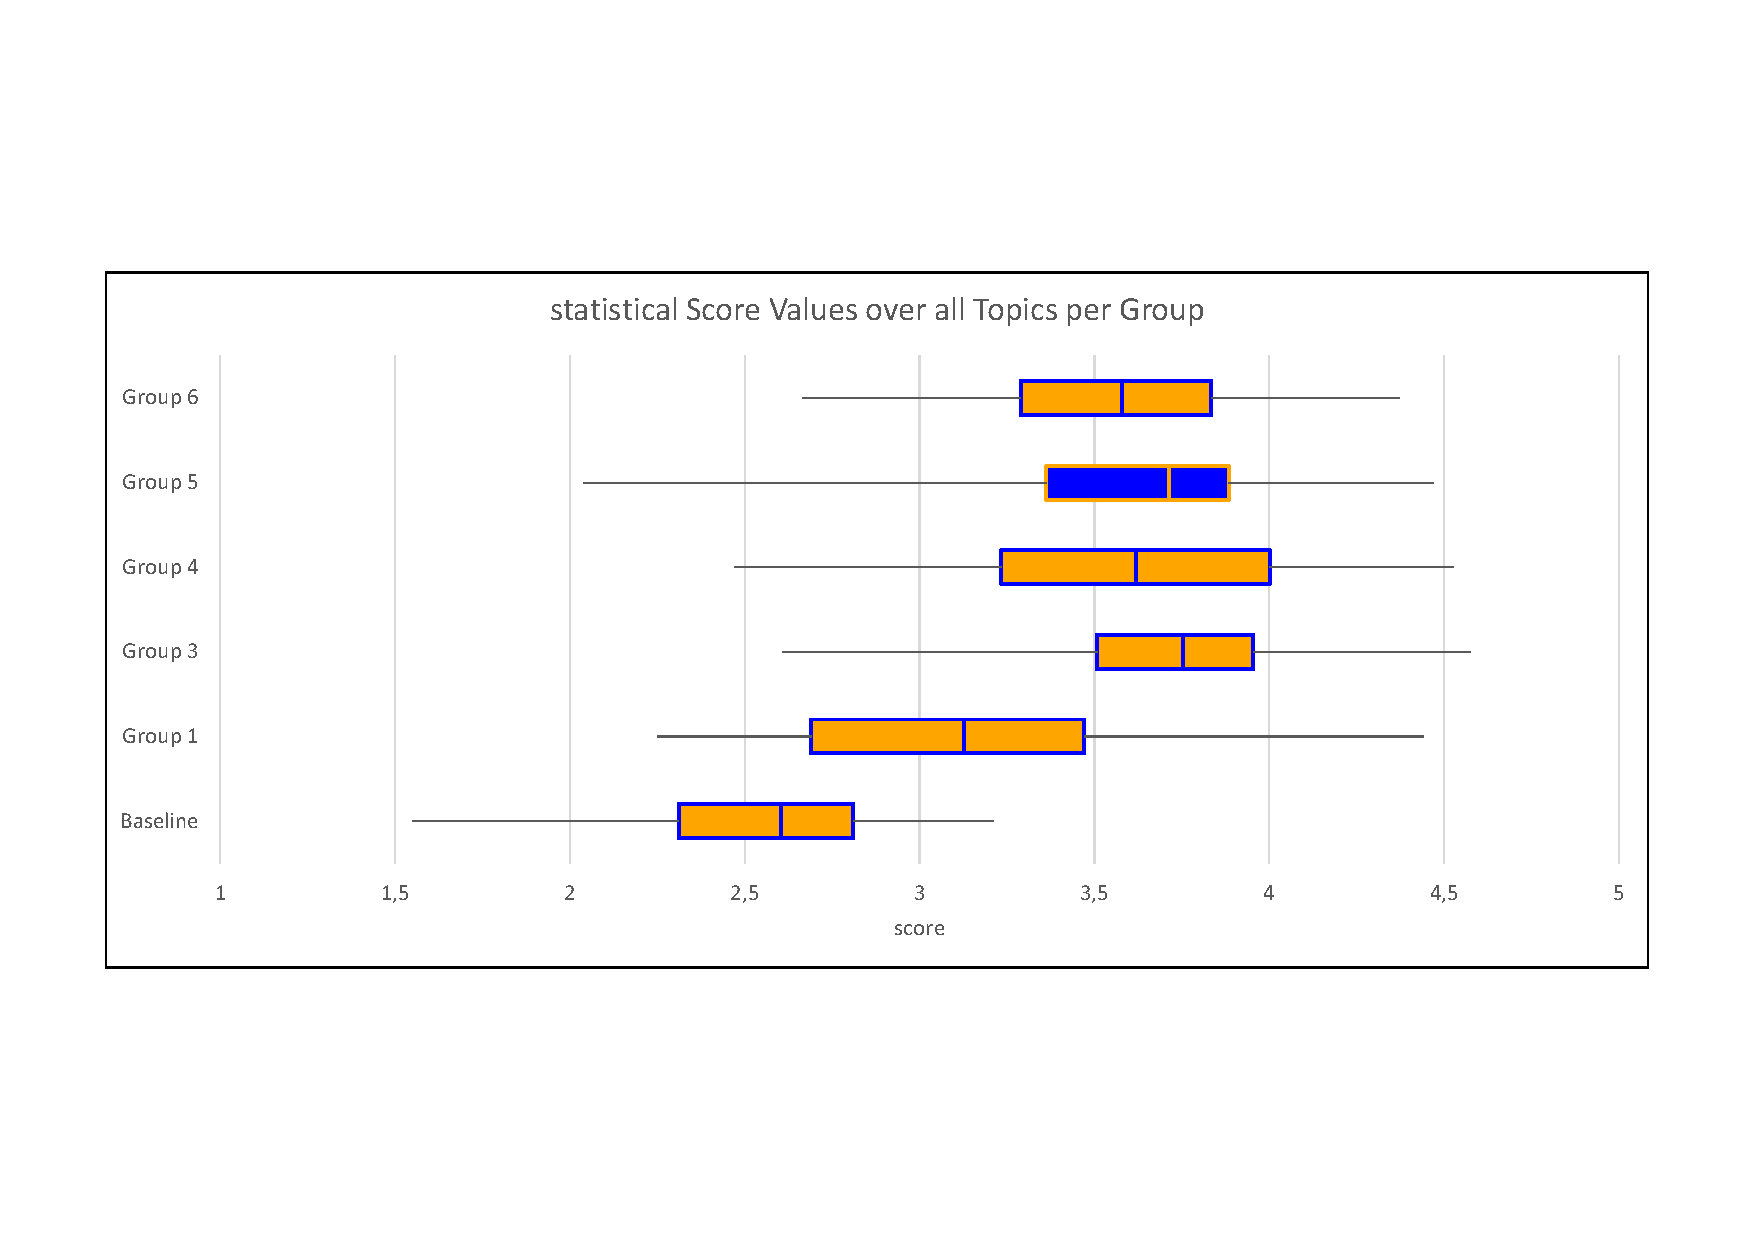
\includegraphics[trim= 0 150 0 150,width=\textwidth]{img/box.pdf}
	\caption{statistical values over all topics per group}
	\label{fig:svg}
\end{figure}


\subsection{Score Calculation with all scales}

\begin{figure}[H]
	\centering
	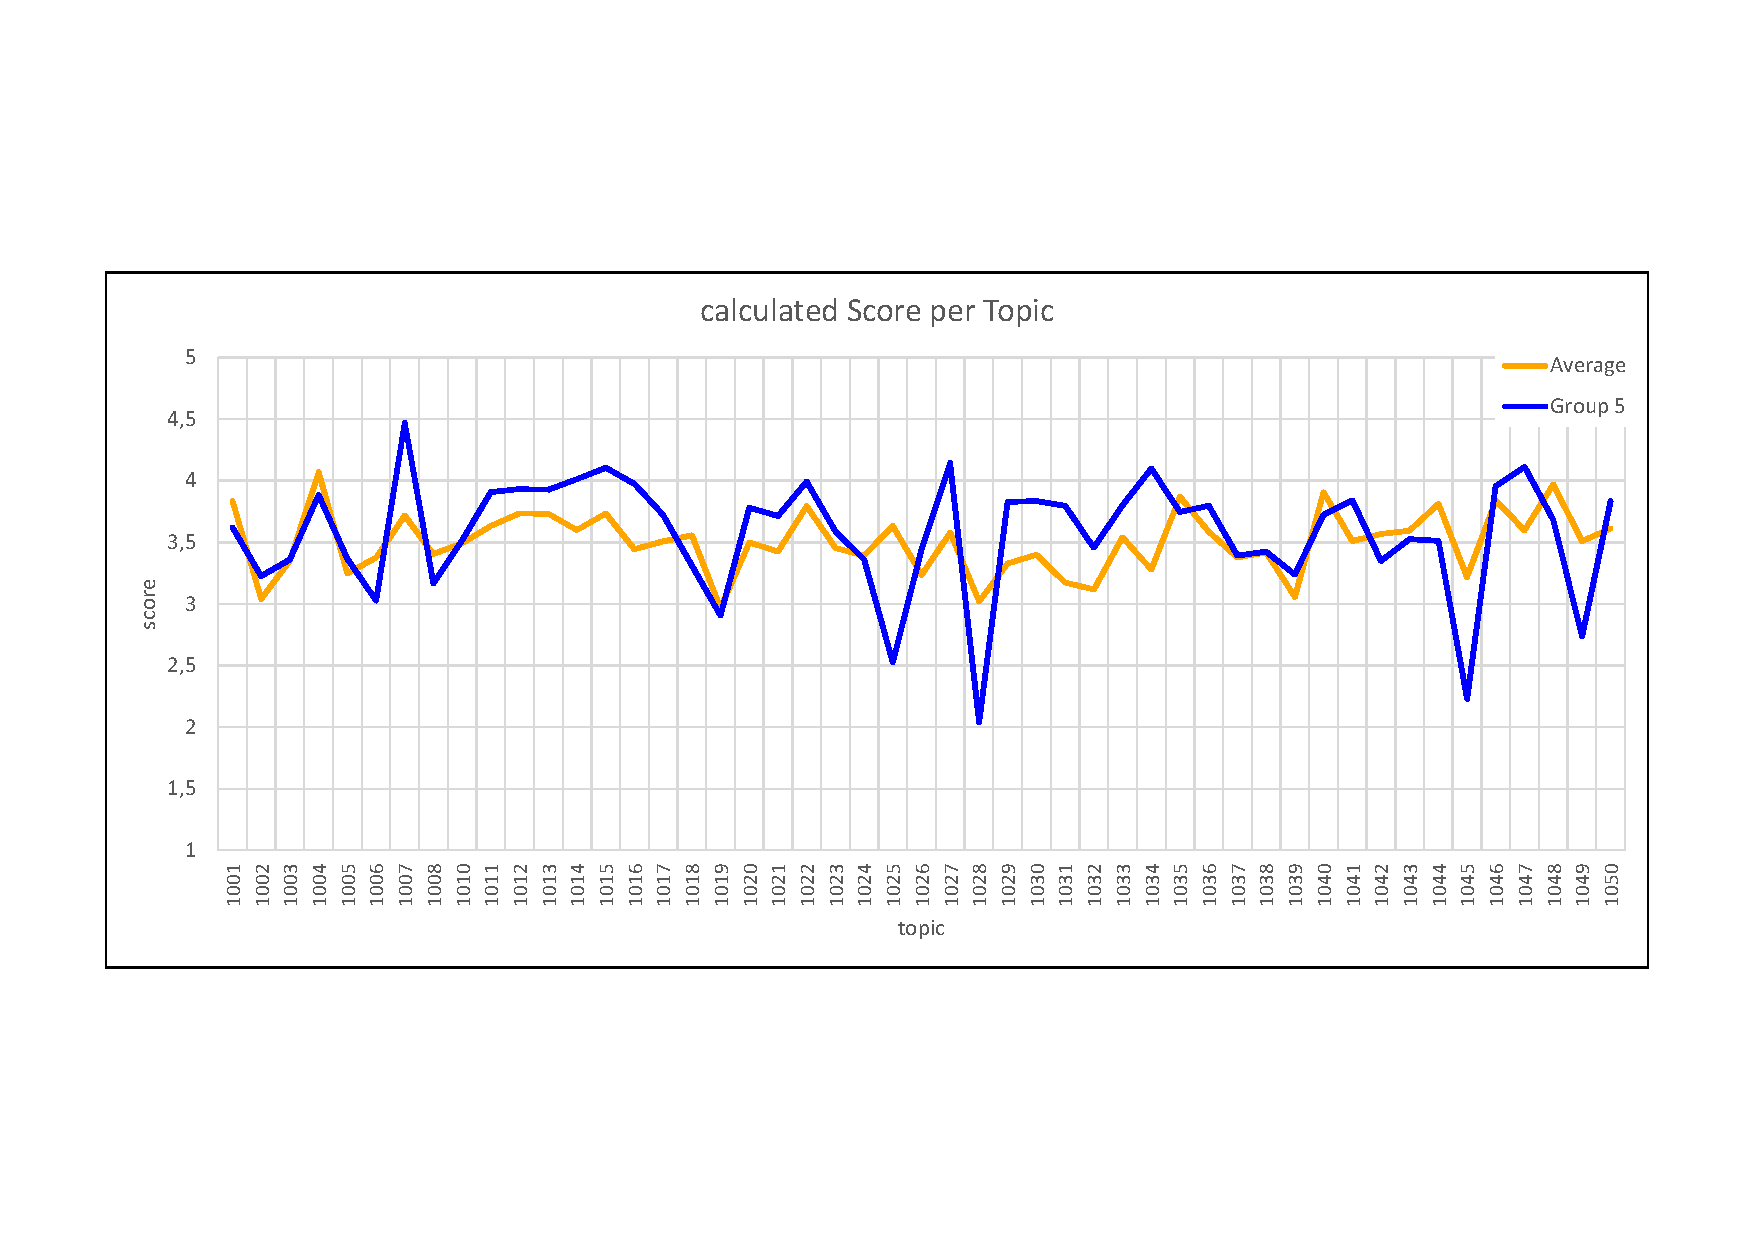
\includegraphics[trim= 0 150 0 150,width=\textwidth]{img/score_per_topic.pdf}
	\caption{scores per topic}
	\label{fig:spt}
\end{figure}


\subsection{calculated score per topic - sorted}

\begin{figure}[H]
	\centering
	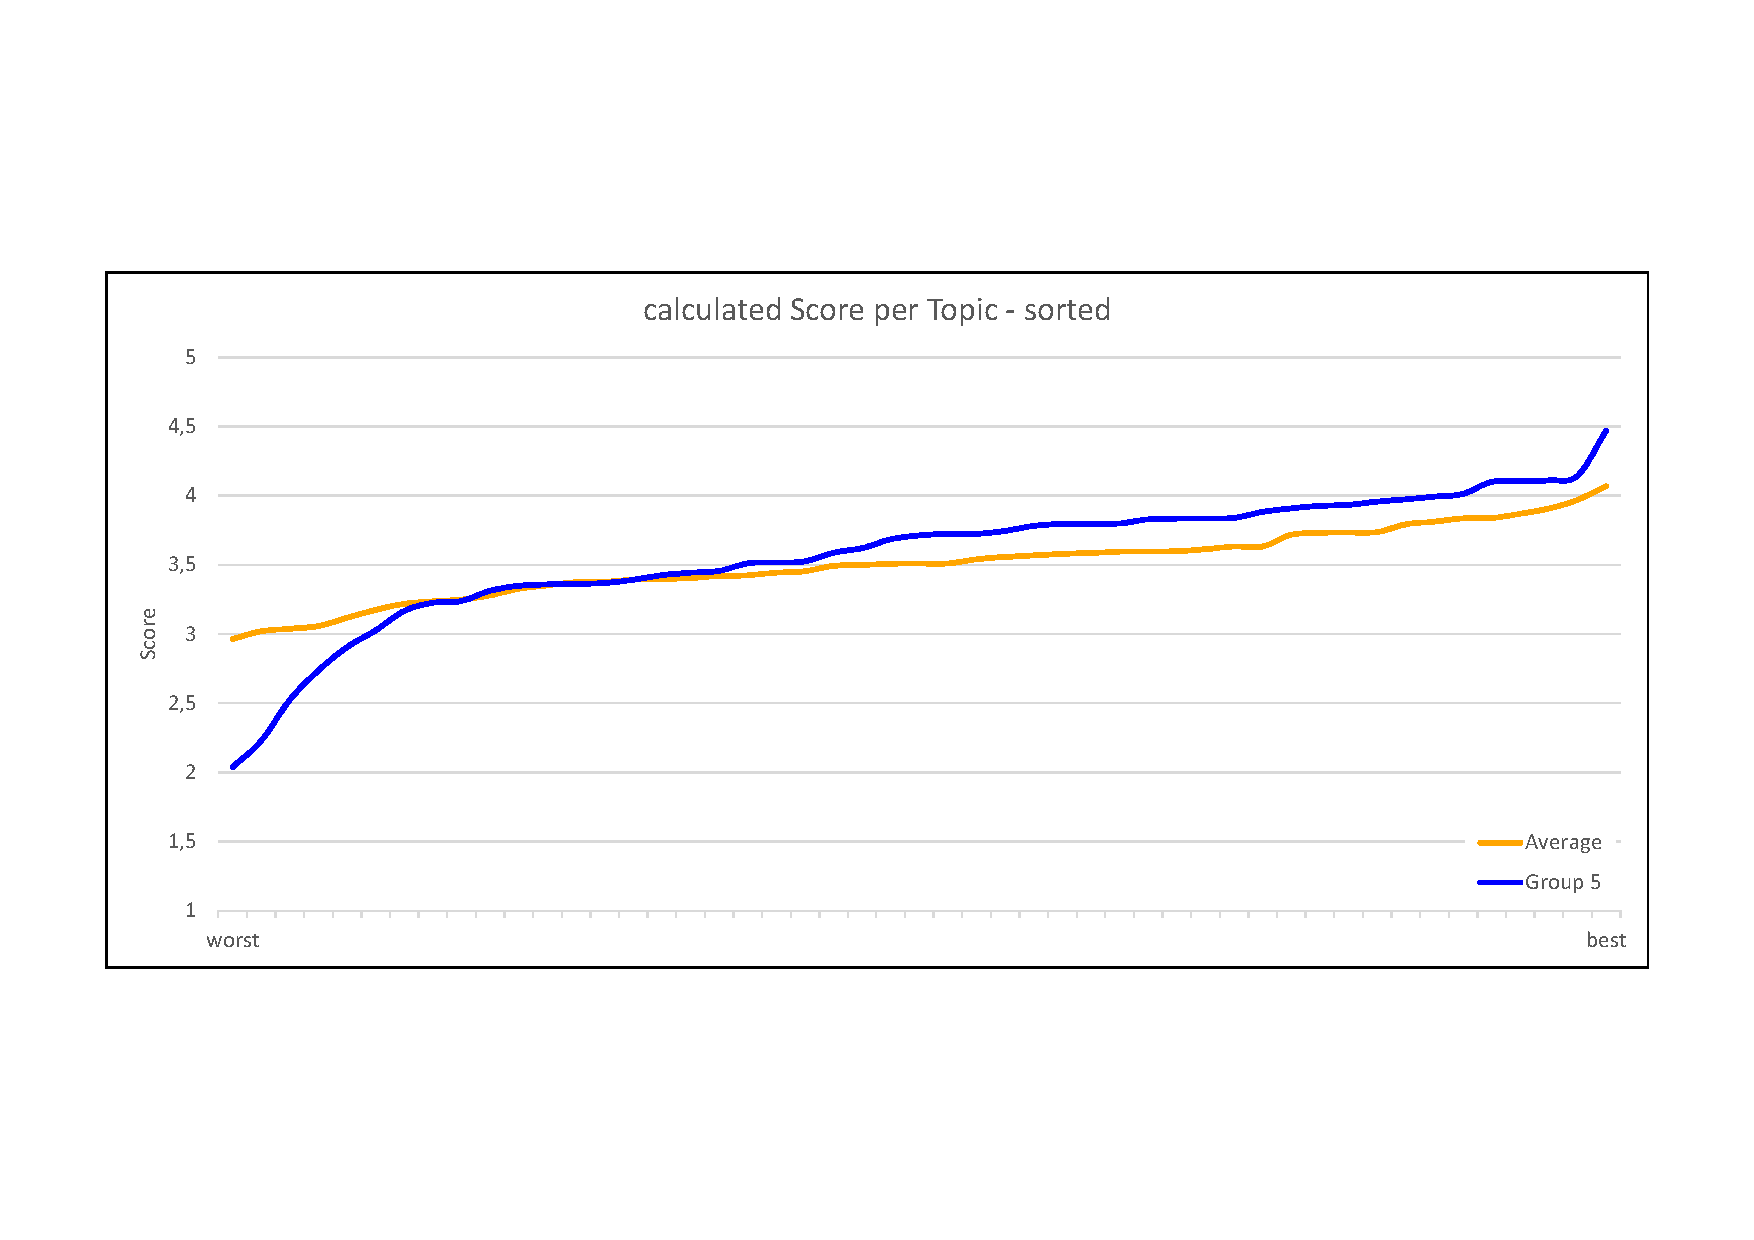
\includegraphics[trim= 0 150 0 150,width=\textwidth]{img/score_per_topic_sorted.pdf}
	\caption{scores per topic sorted ascending}
	\label{fig:spts}
\end{figure}

\subsection{best and worst}